\documentclass[11pt,a4paper]{article}

\usepackage[T1]{fontenc}
\usepackage[utf8]{inputenc}
\usepackage[margin=2.6cm]{geometry}
\usepackage{amsmath,amssymb}
\usepackage{booktabs}
\usepackage{longtable}
\usepackage{graphicx}
\usepackage{array}
\usepackage[table]{xcolor}
\usepackage[colorlinks=true,linkcolor=blue,urlcolor=blue,citecolor=blue]{hyperref}
\usepackage{enumitem}

\newcommand{\PCKP}{\textsc{PCKP}}
\newcommand{\code}[1]{\texttt{#1}}

\title{\textbf{The LP relaxation of the precedence-constrained\\ knapsack problem}\\[2mm]
\large Computational report}
\author{Valerio Dose \and Fabio Furini \and Marco Locatelli}
\date{5 September 2026}

\begin{document}
\maketitle

\begin{abstract}
\noindent
This report documents the software implementation and the experimental study
accompanying our work on the LP relaxation of the precedence-constrained
knapsack problem. It states what was implemented, how each component was
verified, and what the experiments show. The central experimental question is
operational: \emph{how should this relaxation be solved in practice?} The
answer is regime-dependent, and the regime is set by whether one capacity or
the whole value function is needed, and by the density of the precedence
graph --- not by the number of items. A secondary finding concerns accuracy
rather than speed: on one open-pit instance every LP solver we tried returns a
value that is wrong in the eighth significant digit, where the combinatorial
method is exact. The software, the raw measurements and a browsable edition of
this report are at \url{https://github.com/fabiofurini/macroitems}.
\end{abstract}

\tableofcontents
\bigskip

%======================================================================
\section{What was implemented}
\label{sec:implemented}

The library \code{macroitems} (Python, MIT) implements the objects of the
theory and the algorithms that produce them. Everything reduces to maximum
closure, which is one minimum cut on a Picard network.

\subsection{The core}

\begin{longtable}{@{}p{0.30\textwidth}p{0.42\textwidth}p{0.22\textwidth}@{}}
\toprule
\textbf{Function} & \textbf{What it returns} & \textbf{Cost}\\
\midrule
\endhead
\code{max\_closure} & a maximum-value closure, with the inclusion-wise
maximal or minimal tie convention, and optional forcing of items in or out &
one minimum cut\\
\addlinespace
\code{canonical\_path} & the canonical macroitem sequence
$\mathcal I_1,\dots,\mathcal I_k$, its ratios, and hence $z(c)$ for
\emph{every} capacity at once; by geometric bisection or by repeated
maximum-ratio extraction & $O(k)$ maximum flows on shrinking graphs\\
\addlinespace
\code{solve\_capacity} & the LP at one capacity, by a Newton search on the
weight price & a handful of maximum flows\\
\addlinespace
\code{solution\_from\_path} & any capacity read off a precomputed path &
$O(\log k)$, no flow\\
\addlinespace
\code{canonical\_dual} & the canonical dual certificate: the capacity price
and three region-wise flows & three maximum flows\\
\addlinespace
\code{best\_reduced\_costs} & reduced costs optimised over the \emph{whole}
dual optimal face, and the items a given incumbent lets one fix &
one minimum cut per item\\
\addlinespace
\code{face\_dimensions} & dimensions of the primal and dual optimal faces &
$|\mathcal H|$ minimum cuts\\
\addlinespace
\code{first\_macroitem\_lawler} & Lawler's binary search on the ratio, kept
for comparison & $O(\log)$ maximum flows\\
\bottomrule
\end{longtable}

\subsection{Infrastructure}

\begin{description}[leftmargin=1.4em,style=nextline]
\item[Three interchangeable maximum-flow backends.] OR-Tools (int64, exact
and the default), igraph (floating point) and SciPy (int32). They must agree
on integer data, which the test suite checks. SciPy \emph{refuses} capacities
above $2^{31}-1$ rather than truncating them, for the reason in
Section~\ref{sec:defects}.

\item[Exact arithmetic wherever the data allow it.] Instances with decimal
data are scaled to integers by reading the number of decimals off each
value's shortest decimal representation and scaling in decimal arithmetic.
Closures, macroitems and ratios are invariant under that scaling, so the
answer does not change, but the parametric values become integers and the
whole computation is exact: the breakpoints are recovered as rationals and no
tolerance decides which macroitem an item belongs to. Six of the ten MineLib
instances and all 23 benchmark instances enter this regime.

\item[Five LP baselines behind one interface.] HiGHS (the reproducible
open-source reference), SciPy, Gurobi, CPLEX, and a CPLEX backend that drives
a licensed Interactive Optimizer over a pipe --- necessary because the CPLEX
distribution on PyPI is the Community Edition, which refuses models above
1000 rows, that is, every instance considered here. Each builds its model
once and re-solves at further capacities by changing only the capacity
right-hand side, so simplex bases carry over; build time and solve time are
reported separately. \textbf{No third-party solver code is bundled}: the
solvers are linked, and installed by the user under their own licences.

\item[Instance readers.] For MineLib and for the precedence-constrained
knapsack benchmark, in both of the latter's formats. The MineLib tonnage is
determined and \emph{verified} automatically, see Section~\ref{sec:instances}.

\item[A command-line interface and experiment scripts] for the structural
characterisation, the method comparison, the revenue-factor study, and the
generation of every table and figure in this report from the raw CSV files.
\end{description}

\subsection{What was implemented and then disabled}

The reduction of the canonical path to a single source--sink-monotone
parametric minimum cut is implemented and tested, and then deliberately
disabled, because the public implementation it would call is incorrect. See
Section~\ref{sec:parametric}.

%======================================================================
\section{What was tested, and how}
\label{sec:tested}

The suite is 773 tests and runs in about seventy seconds. Its design principle
is that every check has an \emph{independent} reference: exact rational
arithmetic, a second backend, a second algorithm, or the LP itself. That
matters here more than usual, because in this subject a wrong implementation
returns something that looks like an answer --- nested chains of closures,
decreasing ratios, plausible reduced costs.

\subsection{Against an exact brute-force reference}

Small instances are compared against a reference written in exact rational
arithmetic that enumerates \emph{every} closure.

\begin{center}
\begin{tabular}{@{}p{0.55\textwidth}r@{}}
\toprule
\textbf{What is checked} & \textbf{Coverage}\\
\midrule
$u(\lambda)$ and both lattice extremes at every breakpoint & $\sim3\,800$
$(\lambda,\text{instance})$ pairs, 216 instances\\
the canonical sequence, from its definition & 216 instances, both algorithms\\
$z(c)$ over a capacity grid & 136 instances $\times$ a half-integer grid\\
persistency against the \emph{full} optimal face & $1\,700+$ capacities, of
which $250+$ with non-unique optima\\
the dual certificate & 80 instances\\
\bottomrule
\end{tabular}
\end{center}

The degenerate cases are deliberate: all profits negative, all positive, zero
profits, a single item, no arcs, stars, chains, and instances built so that
two disjoint continuations have equal ratio. The tie convention is where this
subject hides its errors.

\subsection{Invariants, on arbitrary instances}

Property-based tests (\code{hypothesis}, $\sim900$ generated instances) assert
what must hold for \emph{any} instance: prefixes are closures; the macroitems
partition the item set; ratios strictly decrease in exact arithmetic; $z(c)$
is concave and nondecreasing; the returned solution is feasible and attains
the reported value.

\subsection{Between implementations}

The two path algorithms must agree (100 random DAGs across five densities and
two seeds, plus grids); the three maximum-flow backends must give identical
closures and paths on integer data; the LP baselines must agree with the
combinatorial methods and with each other to $10^{-9}$; and the integer
rescaling must preserve ratios while scaling values.

\subsection{Against the other literatures}

This is the part that tests the \emph{theory}'s claim rather than the code.
Each algorithm is reimplemented from its own source, using nothing from the
library.

\begin{center}
\begin{tabular}{@{}p{0.26\textwidth}p{0.42\textwidth}p{0.24\textwidth}@{}}
\toprule
\textbf{Source} & \textbf{Claim} & \textbf{Coverage}\\
\midrule
Dantzig (1957) & with no arcs the theory reduces to the greedy ratio rule &
67 arc-free instances\\
\addlinespace
Shaw and Cho (1998) & their aggregated subtrees are the macroitems and their
bound is $z(c)$ & 43 tree instances, $\sim1\,500$ capacities\\
\addlinespace
Sidney (1975); Margot, Queyranne and Wang (2003) & the reduced Sidney
decomposition is the canonical sequence, after reversing the arcs and
swapping the roles of the data & 57 instances, decomposition by brute force
over all initial sets\\
\bottomrule
\end{tabular}
\end{center}

All three hold. They are not vacuous: dropping the arc reversal in the
scheduling translation breaks 188 of 190 instances, and using the finest
rather than the coarsest tie convention in the Shaw--Cho deletion breaks 8 of
the 43 tree cases.

\subsection{As a user receives it}

The package is built as a wheel, installed into an empty environment, and
exercised from the command line, both with all optional backends and with its
declared dependencies alone. Continuous integration runs the suite on Python
3.10 to 3.13 and repeats the core-only installation on every push. Two of the
defects of Section~\ref{sec:defects} were found by exactly this.

%======================================================================
\section{Instances}
\label{sec:instances}

No instance data is redistributed; the readers take the files as published by
their authors.

\begin{center}
\begin{tabular}{@{}llrr@{}}
\toprule
\textbf{Collection} & \textbf{Family} & \textbf{Instances} & \textbf{Sizes}\\
\midrule
\PCKP\ benchmark & telecom (A--K) & 11 & $n=972$--$9\,235$, $m/n\approx1.8$\\
                 & mining (L--W)  & 12 & $n=349$--$11\,757$, $m/n\approx6$--$7$\\
MineLib          &                & 10 & $n=1\,060$--$112\,687$, up to $m=3\,035\,483$\\
\bottomrule
\end{tabular}
\end{center}

Two points about the files are worth recording, since both cost time to
establish.

\paragraph{The MineLib tonnage is not labelled.} The block-model files carry
between 8 and 19 unlabelled attributes and the format specification calls them
"optional user-specified fields". The reader determines the tonnage and
verifies it: every block must be moved, so the tonnage is positive on
\emph{all} blocks; an operational resource of the constrained-pit file whose
coefficients cover every block is therefore the mining resource, and is used
directly (8 of the 10 instances). A resource covering only part of the blocks
is a processing resource, and then the tonnage is the block attribute that is
positive everywhere \emph{and} agrees with those partial coefficients wherever
they exist --- the agreement identifies the column, since a processing
resource charges an ore block exactly its tonnage. This settles \code{kd}
(agreement on all $5\,931$ ore blocks) and \code{mclaughlin\_limit} (on all
$31\,931$). Each instance records how it was decided.

\paragraph{The benchmark's two formats disagree on item numbering.} On 13 of
the 23 instances the LP-format and tabular files number the items
differently. They are the same instances --- the multisets of profits and
weights agree exactly, and so do the arc counts --- but item indices are not
comparable across formats. Separately, the family labels in the
\code{runList} files distributed with some copies of the accompanying code
are the opposite of the original distribution's; the data settle it, since
the mining instances are the ones with negative-profit waste.

%======================================================================
\section{Setup and protocol}
\label{sec:setup}

Intel Core i5-14500T, 14~GB, Ubuntu 26.04, Python 3.14.4; OR-Tools 9.15,
igraph 1.0, HiGHS 1.15.1, Gurobi 13.0.3, CPLEX 22.1 (Interactive Optimizer,
licensed).

Every run is single-threaded. Each method runs in its own process --- required
for correctness, since \code{highspy} and \code{ortools} export incompatible
copies of the same C\texttt{++} symbols and only the one imported first
loads, and good practice for timing in any case. Build time is separated from
solve time, and the LP baselines build once and then change only the capacity
right-hand side, so their simplex bases carry over; a baseline that rebuilt
its model at every capacity would be measuring the wrong thing. Capacities
are evenly spaced inside $(0,w(\mathcal M_q))$, the range on which the
capacity constraint binds. Every method's values are compared against the
canonical path at every capacity, and any relative difference above $10^{-9}$
is reported rather than hidden.

%======================================================================
\section{The structure of real instances}
\label{sec:structure}

The fraction $1-|\mathcal H|/n$ of items whose value is the same in every
optimal solution --- the persistency --- is what the relaxation settles on its
own. It varies enormously.

\begin{center}
\begin{tabular}{@{}llrl@{}}
\toprule
 & \textbf{Instance} & \textbf{Persistency} & \textbf{Split macroitem}\\
\midrule
lowest  & O\_1711\_11661 & 0.150 & $1\,455$ of $1\,711$ items\\
        & newman1        & 0.166 & $884$ of $1\,060$ blocks\\
        & U\_6494\_48626 & 0.262 & $4\,790$ of $6\,494$\\
highest & p4hd           & 0.992 & $329$ of $40\,947$\\
        & sm2, zuck\_large & 0.9999 & $10$ of ${\sim}100\,000$\\
\bottomrule
\end{tabular}
\end{center}

On \code{sm2} and \code{zuck\_large} the relaxation fixes all but ten blocks
out of a hundred thousand; on \code{newman1} it fixes almost nothing. This is
the \emph{gap problem} of the mining literature, measured rather than
described, and the theory says exactly what separates the two groups: the
weight of the split macroitem relative to the capacity.

\begin{figure}[htbp]
\centering
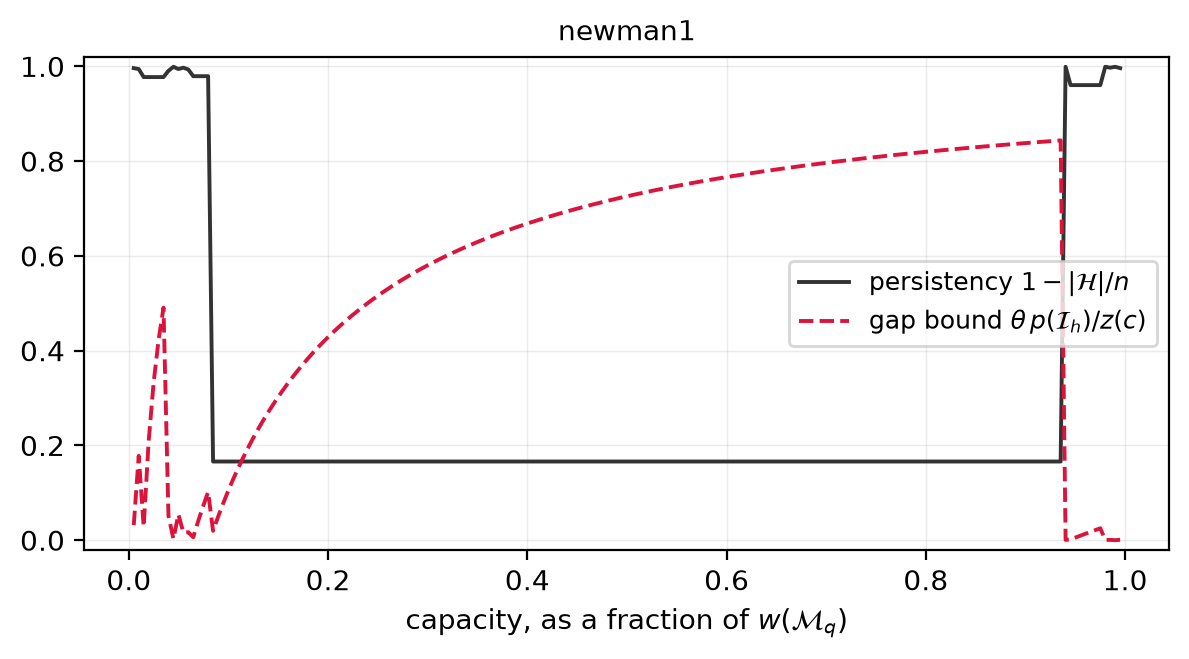
\includegraphics[width=0.86\textwidth]{../experiments/results/figures/newman1_persistency.png}
\caption{Persistency and the integrality-gap bound across the capacity range
of \code{newman1}. Persistency is near 1 only below 8\% of
$w(\mathcal M_q)$; over the entire practical range it collapses to $0.166$
while the gap bound climbs to $0.84$. One macroitem dominates the instance.}
\end{figure}

\paragraph{The published capacities sit in the hard regime.} On \emph{all} 23
benchmark instances the distributed capacity is between 0.5\% and 25\% of
$w(\mathcal M_q)$, so the split macroitem is the \emph{first} one. The
optimal solution is then a multiple of a single macroitem's indicator, the
integrality-gap bound is vacuous, and the true gap against the known integer
optima is large: median 26.6\%, up to 85.6\%. The standard benchmark of this
problem exercises precisely the regime in which the natural relaxation is
weakest, which is consistent with that literature's focus on cutting planes.

%======================================================================
\section{How best to solve the relaxation}
\label{sec:methods}

\subsection{The whole value function}

The canonical path returns \emph{every} capacity at once; a further capacity
then costs a binary search over the breakpoints. An LP solver answers one
capacity per solve. Over twenty capacities on the benchmark, against the
fastest of the three simplex codes:

\begin{center}
\begin{tabular}{@{}lrrl@{}}
\toprule
\textbf{Group} & \textbf{Instances} & \textbf{Median ratio} & \textbf{Range}\\
\midrule
sparse, $m<10^4$        & 12 & $1.00\times$ & 0.47--2.44\\
dense, $m\ge2\cdot10^4$ &  7 & $\mathbf{11.2\times}$ & 5.0--29.0\\
\bottomrule
\end{tabular}
\end{center}

The largest benchmark instance, $n=11\,757$ and $m=83\,218$, takes $0.42$
seconds for the whole of $z(\cdot)$ against $12.2$ seconds for one grid of
solves, a factor of 29.

\paragraph{Density, not size, is the discriminant.} The sparse group contains
instances with $9\,235$ items on which the methods tie, while an instance with
$3\,243$ items but $22\,306$ arcs already gives a factor of 8. What separates
them is the precedence structure a simplex basis has to carry.

On the open-pit instances the effect is larger. On \code{zuck\_small}
($9\,400$ blocks, $145\,640$ precedences) the path returns the entire value
function in $0.58$~s against $26.3$~s for the fastest solver over twenty
capacities; on \code{zuck\_medium} ($29\,277$ blocks, $1\,271\,207$
precedences) in $3.45$~s against $1\,355$~s for HiGHS dual simplex, a factor
of 390 --- and under a 420~s per-method budget HiGHS does not finish that
instance at all.

\subsection{One capacity}

The Newton search on the weight price is a median $1.5\times$ faster than the
fastest simplex code, with a wide range ($0.38$--$26.9\times$): on small
sparse instances a warm-started dual simplex is at least as good, and there
is no reason to prefer the combinatorial route there.

\subsection{Interior point}

Barrier and IPM cannot start from a previous basis, so their marginal cost per
capacity equals their full cost; over a grid they were 10--30 times worse than
dual simplex in every run, and they are the first to hit a time limit on the
large instances. Worth stating, because barrier is a common default on large
sparse LPs and here it is the wrong default.

\subsection{Recommendation}

\begin{center}
\begin{tabular}{@{}p{0.30\textwidth}p{0.30\textwidth}p{0.32\textwidth}@{}}
\toprule
\textbf{Situation} & \textbf{Use} & \textbf{Why}\\
\midrule
one capacity, sparse graph & either & they tie\\
one capacity, dense graph & Newton on the weight price & a handful of cuts on
shrinking graphs\\
more than a couple of capacities & the canonical path & further capacities are
free\\
an LP solver is required & dual simplex, never barrier & only simplex warm
starts\\
the value must be exact & the combinatorial method & Section~\ref{sec:accuracy}\\
\bottomrule
\end{tabular}
\end{center}

%======================================================================
\section{Accuracy}
\label{sec:accuracy}

Across 161 method-runs on the 23 benchmark instances, twenty capacities each,
the largest relative difference between any two methods is
$4.8\cdot10^{-11}$.

On MineLib \code{kd} it is not. At one capacity out of twenty, all five LP
solver configurations return $220\,239\,941.533204$ where the exact value,
computed in rational arithmetic from the integer-scaled instance, is
\[
\frac{1\,238\,890\,176\,810\,816\,816\,310\,940\,159}{5\,625\,184\,000\,000}
= 220\,239\,938.251054 ,
\]
a relative error of $1.5\cdot10^{-8}$ where at the other nineteen capacities
the same solvers agree to $10^{-15}$. It is not an artefact of the integer
rescaling: Gurobi returns the same wrong value on the original decimal data.
The instance has profits of order $4\cdot10^5$ against weights of order
$10^4$, and at that capacity it is ill-conditioned enough for a
double-precision solver's default tolerances.

An error of $10^{-8}$ is harmless when the LP value is a report. It is not
harmless when it is a \emph{bound}: inside an enumerative algorithm a bound
too large prunes nothing it should, and a bound too small prunes an optimal
subtree. Nor is it harmless when the quantity of interest is a difference of
two LP values, as an integrality gap or a reduced cost is. This is the
argument for the combinatorial route that a table of running times does not
show.

%======================================================================
\section{Dual certificates and reduced costs}

The canonical dual certificate is three maximum flows, one per region, and
costs about as much as the primal solution. On every instance it was feasible
and complementary to machine precision --- a meaningful check, since the
feasibility conditions of the three flow systems are exactly the optimality of
the two extremal closures together with the maximum-ratio property of the
split macroitem, so a failure would indicate an error in the \emph{primal}.

Reduced costs optimised over the whole dual optimal face need one minimum cut
per item: for a null item, a maximum closure on the subgraph induced by the
null region with that item forced in; for a full item, the same computation on
the full region \emph{with the arcs reversed}, since a co-closed set of a
graph is a closed set of its reverse. The two cases minimise different
objectives, and confusing them yields bounds that are invalid but entirely
plausible (Section~\ref{sec:defects}).

The face-wide values are never smaller than the closed-form canonical ones
$w_i|\lambda_r-\lambda_h|$, and on the running example they are exactly twice
as large on every item outside the split macroitem; the gain grows with the
density of the precedence graph. Since a reduced cost fixes a variable when it
exceeds the gap to an incumbent, a larger reduced cost fixes strictly more.
Both quantities were validated against the exact loss obtained by re-solving
the relaxation with each item forced to its opposite bound; over twelve
instances, no violation.

%======================================================================
\section{Parametric implementations}
\label{sec:parametric}

The natural third family of methods is a parametric minimum cut returning all
breakpoints in one computation. We intended to include it and cannot.

The public \code{pseudoflow} package states in its own documentation that it
is a simplified variant of parametric HPF, without free runs or warm starts,
and "should not be used" for comparison with the full algorithm. More
seriously, it \emph{silently returns an incomplete parametric family}. The
smallest failing instance has three items, no precedence arcs, profits
$(3,2,1)$ and unit weights, whose canonical sequence is
$\{1\},\{2\},\{3\}$ with ratios $3>2>1$: it reports two intervals instead of
three, and the set returned for the interval containing $\lambda=7/2$ has
value $-1/2$, so it is not a minimum cut. Failures begin at $n=13$ and are
common by $n=200$.

What makes this dangerous is that the output looks correct: the family
returned is always nested, complete, and made of genuine closures with
decreasing ratios --- a \emph{coarsening} of the canonical sequence. Detecting
the defect costs one maximum closure per macroitem, which is recomputing the
answer by another method. We therefore report no row for it. There is likewise
no public implementation of the Gallo--Grigoriadis--Tarjan algorithm that we
would trust for benchmarking, so published running times for parametric
minimum cut on this problem are difficult to reproduce independently.

One correction to the textbook reduction, found while implementing it: the
offset $K\ge\max_i(-p_i)$ usually quoted does not suffice. The parameter range
must reach below the smallest ratio, which is negative whenever some
$p_i/w_i$ is, and the sink capacity $\lambda w_i+K$ then goes negative, at
which point the underlying C library terminates the process.

%======================================================================
\section{Weight against revenue factor}

Nested pits are usually generated in practice by scaling revenue at fixed
cost. That family is nested too, but it is a different family, and only the
weight parameterisation solves the relaxation of a tonnage-constrained
problem. On block models whose revenue and cost are known by construction,
over a grid of twenty revenue factors, only 5 of 20 revenue-factor pits
coincide with a canonical closure, and the relative symmetric difference to
the canonical closure of the nearest tonnage reaches $0.37$: more than a third
of the blocks differ between the two pits of the same size.

Repeating this on MineLib is blocked by the data rather than the method: the
ultimate-pit and constrained-pit files give a single value per block, from
which revenue and cost cannot be separated; only the production-scheduling
formulation lists a value per destination.

%======================================================================
\section{Defects found during development}
\label{sec:defects}

Recorded because the same failure modes are available to anyone
reimplementing these classical algorithms, and because \emph{every one of them
produced a plausible answer rather than an error}.

\begin{enumerate}[leftmargin=1.6em]
\item \textbf{Reduced costs, sign inverted on the full region.} The two
regions minimise different objectives; getting the second wrong produced
reduced costs that were positive, sensibly ordered and of the right magnitude,
and invalid. Caught by comparing against the exact loss.

\item \textbf{An infeasible point at $c=0$.} A negative Python slice wrapped
around and returned all but the last macroitem --- positive weight for zero
capacity. Caught by property-based testing at the boundary.

\item \textbf{The SciPy maximum-flow backend truncated silently.} It computes
in int32 and truncates larger capacities without warning, returning a
\emph{different canonical path} on integer data with wide coefficients. Caught
by requiring the three backends to agree; such capacities are now refused.

\item \textbf{Ratios divided by the integer scale.} A ratio is invariant under
rescaling; the cumulative profits and weights are not. Reporting code divided
them anyway, which would have published breakpoints wrong by orders of
magnitude with every other number in the same table looking right. Caught by
drawing a figure and noticing the colour bar.

\item \textbf{The package did not install.} A deprecated licence classifier
alongside a modern licence expression makes the build back end refuse the
project outright. Caught by building a wheel and installing it.

\item \textbf{Declared dependencies were not sufficient.} The dual certificate
and the face dimensions used floating-point node values that only an optional
backend accepts. The remedy was not a new dependency but exactness: on integer
data the multiplier is the rational $p(\mathcal H)/w(\mathcal H)$, so
multiplying the node values by $w(\mathcal H)$ makes them integers without
changing which sets are optimal or tight. Caught by a continuous-integration
job on its first execution.
\end{enumerate}

The pattern is worth naming. In this subject a broken implementation returns
something that looks like an answer. The only checks that caught anything were
those with an independent reference: exact rational arithmetic, another
backend, another algorithm, or the LP itself.

%======================================================================
\section{Reproducing this report}

\begin{verbatim}
git clone https://github.com/fabiofurini/macroitems && cd macroitems
pip install -e ".[experiments]"
pytest -q                                        # 773 tests

python experiments/characterize.py    <instances> --out .../characteristics.csv
python experiments/compare_methods.py <instances> --capacities 20 --out .../compare.csv
python experiments/revenue_factor.py  grid:20x20x8:5:1 --factors 20
python experiments/make_tables.py
python experiments/make_figures.py    <instances>
\end{verbatim}

Timings depend on the machine. The \emph{values} do not: any relative
difference above $10^{-9}$ between two methods is flagged in the output, and
if it is not the \code{kd} case of Section~\ref{sec:accuracy} it is a defect,
in this library or in a solver, and we would like to hear about it.

\end{document}
